\documentclass[a4paper,11pt]{article}

\author{David Maldonado, $\href{mailto:david.m.maldonado@gmail.com}%
{david.m.maldonado@gmail.com}$}
\title{Boolos and Jeffrey - HW3}

\usepackage{amsmath}
\usepackage{amssymb}
\usepackage{amsthm}
\usepackage{bussproofs}
\usepackage{cite}
\usepackage[pdftex]{hyperref}
\usepackage{latexsym}
\usepackage{listings}
\usepackage{synttree}
\usepackage{textcomp}
\usepackage{verbatim}
\usepackage{tabu}
\usepackage{tikz}
\usetikzlibrary{trees}
\usetikzlibrary{arrows, automata}
\usepackage[latin1]{inputenc}

\newtheorem{lem}{Lemma}[section]
\newtheorem{thm}{Theorem}[section]
\newtheorem{con}{Conclusion}[section]

\renewcommand\thesection{\Alph{section}}

\begin{document}

\maketitle

\bigskip

% QUESTION 1

\section{} (covered in meeting)

% QUESTION 2

\section{Go with the flow, man...}

\subsection{unary subtraction}

	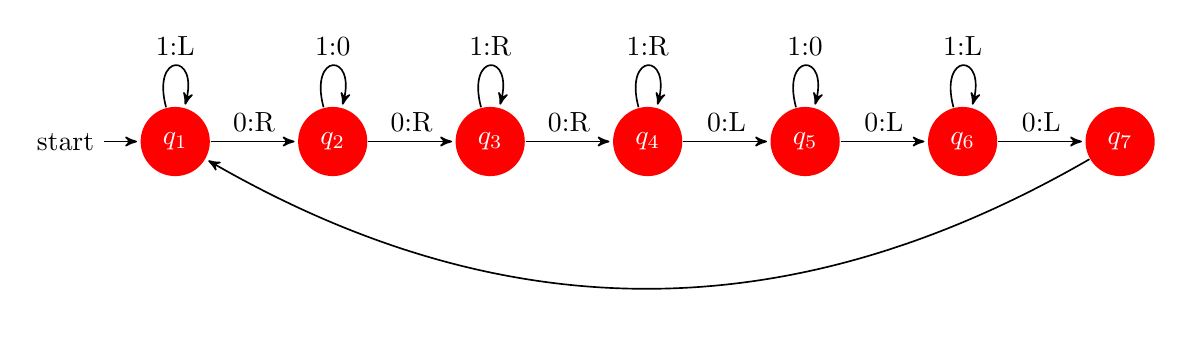
\begin{tikzpicture}[->,>=stealth',shorten >=1pt,auto,node distance=2cm,semithick]
		\tikzstyle{every state}=[fill=red,draw=none,text=white]
		
		\node[initial,state] (A)		{$q_1$};
		\node[state] (B) [right of=A] 	{$q_2$};
		\node[state] (C) [right of=B]	{$q_3$};
		\node[state] (D)	[right of=C]	{$q_4$};
		\node[state] (E) [right of=D] 	{$q_5$};
		\node[state] (F) [right of=E]	{$q_6$};
		\node[state] (G)	[right of=F]	{$q_7$};
		
		\path (A) edge [loop above]	node {1:L} (A)
			       edge 				node {0:R} (B)
			 (B) edge [loop above]	node {1:0}  (B)
			       edge				node {0:R} (C)
			 (C) edge [loop above]	node {1:R}  (C)
			       edge				node {0:R} (D)
			 (D) edge [loop above]	node {1:R}  (D)
			       edge				node {0:L} (E)
			 (E) edge [loop above]	node {1:0}  (E)
			       edge				node {0:L} (F)
			 (F) edge [loop above]	node {1:L}  (F)
			       edge				node {0:L} (G)			 
			 (G) edge [bend left]		node {} (A);

	\end{tikzpicture}
	I think this is heading in the right direction except it never stops!

\subsection{}

\subsection{}
	
\end{document}